\documentclass{beamer}
\usepackage[ngerman]{babel}
\usepackage[utf8]{inputenc}
\usepackage{graphicx}

\usetheme{Singapore}
\usecolortheme{crane}

\title{git}
\author{Johannes Held}
\date{10.05.2010}

\begin{document}

\frame{\titlepage}

\frame{\tableofcontents}

\section{Einleitung}
\frame{
	\frametitle{Einleitung}
	\begin{block}{Wozu brauchen wir GUI?}
		\begin{itemize}
			\pause
			\item einfacher
			\pause
			\item dynamischer
			\pause
			\item schöner
		\end{itemize}
	\end{block}
}

\frame{
\tableofcontents
}


\section{DVCS}
\frame{
	\frametitle{DVCS}
}

\subsection{workflows}
\frame{
	\frametitle{workflows - zentralisiert}
	\begin{figure}[h]
		\center
		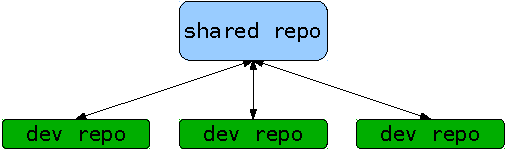
\includegraphics{pics/workflow_01.pdf}	
	\end{figure}
}

\frame{
	\frametitle{workflows - integriert}
	\begin{figure}[h]
		\center
		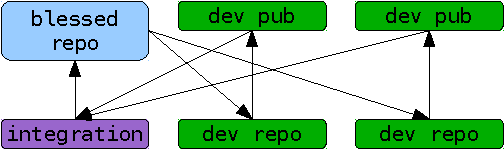
\includegraphics{pics/workflow_02.pdf}	
	\end{figure}
}

\frame{
	\frametitle{workflows - diktatur}
	\begin{figure}[h]
		\center
		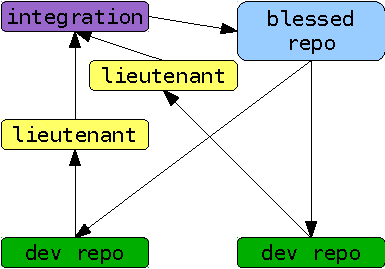
\includegraphics{pics/workflow_03.pdf}	
	\end{figure}
}

\section{git}
\frame{
	\frametitle{git}
}

\subsection{init and commit}
\frame{
	\frametitle{init}
}

\subsection{branch}
\frame{
	\frametitle{branch}
	\begin{figure}[h]
		\center
		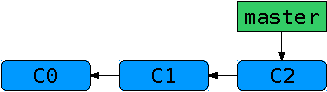
\includegraphics{pics/branch_01.pdf}	
	\end{figure}
}

\frame{
	\frametitle{branch}
	\begin{figure}[h]
		\center
		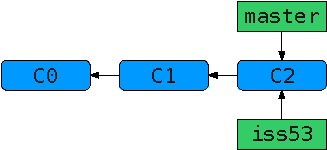
\includegraphics{pics/branch_02.pdf}	
	\end{figure}
}

\frame{
	\frametitle{branch}
	\begin{figure}[h]
		\center
		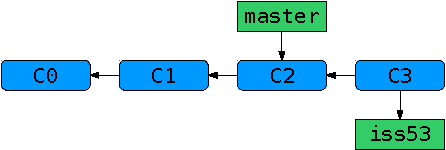
\includegraphics{pics/branch_03.pdf}	
	\end{figure}
}

\frame{
	\frametitle{branch}
	\begin{figure}[h]
		\center
		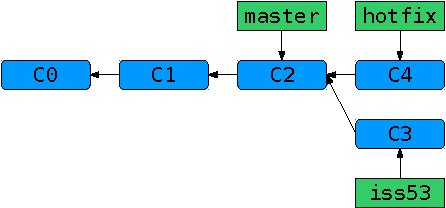
\includegraphics{pics/branch_04.pdf}	
	\end{figure}
}

\subsection{merge}
\frame{
	\frametitle{merge}
	\begin{figure}[h]
		\center
		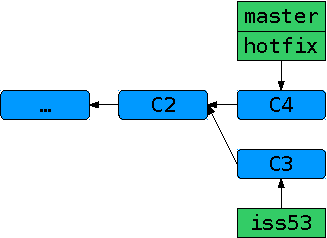
\includegraphics{pics/merge_01.pdf}	
	\end{figure}
}

\frame{
	\frametitle{merge}
	\begin{figure}[h]
		\center
		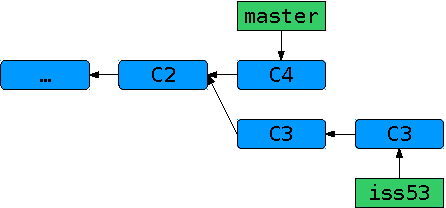
\includegraphics{pics/merge_02.pdf}	
	\end{figure}
}

\frame{
	\frametitle{merge}
	\begin{figure}[h]
		\center
		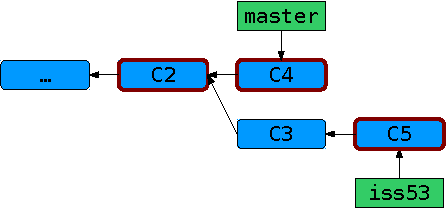
\includegraphics{pics/merge_03.pdf}	
	\end{figure}
}

\frame{
	\frametitle{merge}
	\begin{figure}[h]
		\center
		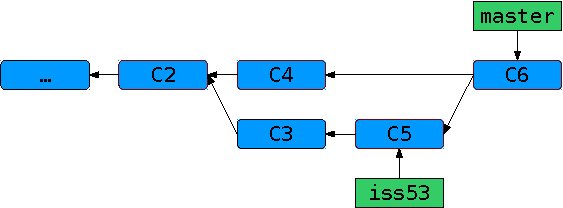
\includegraphics{pics/merge_04.pdf}	
	\end{figure}
}

\subsection{rebase}
\frame{
	\frametitle{rebase}
	\begin{figure}[h]
		\center
		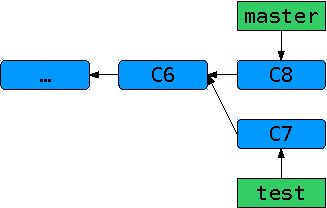
\includegraphics{pics/rebase_01.pdf}	
	\end{figure}

}

\frame{
	\frametitle{rebase}
	\begin{figure}[h]
		\center
		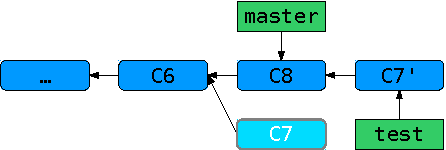
\includegraphics{pics/rebase_02.pdf}	
	\end{figure}

}

\frame{
	\frametitle{rebase}
	\begin{figure}[h]
		\center
		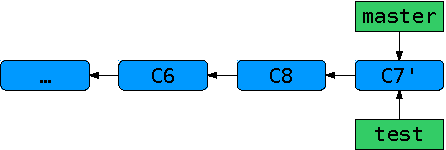
\includegraphics{pics/rebase_03.pdf}	
	\end{figure}

}

\section{diff to others like hg}
\frame{
	\frametitle{diff }
}

\section{Mehr Informationen}
\frame{
	\frametitle{Mehr Informationen}
	\begin{block}{Webseiten}
		 http://whygitisbetterthanx.com/
		\\ http://progit.org
		\\ \small{http://versioncontrolblog.com/comparison/Git/Mercurial/index.html}
		\\ http://www.gitready.com/
		\\ http://git-scm.com/
	\end{block}

	\begin{block}{Dieser Foliensatz}
		git clone git://github.com/hehejo/NTDM-GIT.git
	\end{block}
}


\end{document}
